\subsubsection{Backend}
Mit Beginn der Backend-Entwicklung wurden in erster Linie die Grundstrukturen implementiert, um der \textit{MVVM}-Architektur gerecht zu werden. Dabei lag 
der Fokus bei der Instanziierung der notwendigen Komponenten auf der \textit{Android Architecture Components}. Nach chronologischer Reihenfolge wurden die Klassen 
erstellt und mit den dazugehörigen Funktionen und Methoden versehen. Angefangen wurde mit der Entity-Klasse zur Beschreibung des Objekts und deren allgemeinem Aufbau, 
wie bereits in der Konzeption (\ref{chap:Konzeption}) unter dem Datenmodell (\ref{chap:Datenmodell}) festgehalten. Darauffolgend wurde das „Data Object“ 
erstellt, welches die Zugriffe der Datenbankobjekte verwaltet. Abschließend wird im Bereich der Datenbank ein Room-Layer eingebaut, um die eigentliche Datenbank zu 
instanziieren und eine Zugriffsschicht auf diese zu implementieren. 
\\ 
Zur Modularisierung und Generierung einer Schnittstelle zur Kommunikation zwischen einzelnen Datenbeziehungspunkten und der Datenbank wurde ein Repository erstellt, 
das aus verschiedenen Quellen Daten zusammenbringen kann und eine saubere \acs{API} für den Datenzugriff auf den Rest der Anwendung bietet. 
Um die vorhandenen Klassen zum Datentransfer und zum Persistieren der Daten mit der eigentlichen Benutzeroberfläche zu verbinden, wurde ein ViewModel implementiert, 
welches die Daten zwischen den einzelnen Komponenten teilt und bereitstellt. 
\\ 
\linebreak 
Nach Aufzählung der einzelnen Bestandteile wird auf diese genauer eingegangen. 
\\ 
\linebreak
In einer Java-Klasse wird mithilfe der gegebenen Bibliothek „Room“ ein Entity-Objekt erstellt. Hierbei gibt es eine eindeutige Annotation, die die Klasse und 
deren beinhalteten Variablen deklariert. In dem folgend aufgeführten Code-Beispiel (\ref{code:entity}) ist diese Annotation zu entnehmen, dabei ist die Klasse als 
Entity deklariert und wird somit in eine Datenbank-Tabelle konvertiert. 
In dieser Tabelle, bezeichnet als \textit{„object\_table“}, gibt es weitere Variablen, die zuerst mit Annotationen versehen und dann gemäß der Anforderungen des 
Konzepts definiert sind. Diese Variablen repräsentieren die Attribute des Datenbankschemas und stellen die einzelnen 
Informations-, bzw. Datenbankspalten dar. Zur Veranschaulichung dient die Initialisierung der \acs{ID}-Vergabe eines Objekts. Diese wird als \textit{„id“}-Spalte 
und ebenso als Primärschlüssel\footnote{Ein Wert einer Tabelle, bzw. eines Attributs, der den Tabelleneintrag eindeutig identifiziert.}-Variable 
deklariert.
\\ 
%\linebreak
\begin{lstlisting}[language=C,
    frame=lines,           % Ein Rahmen um den Code (single for box, lines for top and bottom)
    xleftmargin=\parindent,  % Rahmen link von den Zahlen
    style=algoBericht,
    label={code:entity},
    captionpos=b,           % Caption unter den Code setzen
caption={Entity Code zur Initialisierung der Objekte}]
@Entity(tableName = "object_table")
public class Object {
    @ColumnInfo(name = "id")
    @NonNull
    @PrimaryKey(autoGenerate = true)
    private int id;

    public int getId() { return this.id; }
    public void setId(int id) { this.id = id; }
    ... 
}
\end{lstlisting}
\pagebreak
Das mit der Entity-Klasse kommunizierende Modul ist das \textit{„Data Object“}, welches als Interface angelegt wurde. Das „Object Dao“ verwendet ebenso die Bibliothek 
„Room“ und wandelt die Java-Klasse per Annotation in ein „Dao“ um. Dieses beinhaltet hauptsächlich die SQL-Queries zur Datenabfrage der vorhandenen Informationen. 
\\
%\linebreak
\begin{lstlisting}[language=C,
    frame=lines,           % Ein Rahmen um den Code (single for box, lines for top and bottom)
    xleftmargin=\parindent,  % Rahmen link von den Zahlen
    style=algoBericht,
    label={code:query},
    captionpos=b,           % Caption unter den Code setzen
caption={SQL-Query zur Abfrage der Objekt-Namen}]
@Query(SELECT * FROM object_table ORDER BY name)
LiveData<List<Object>> getObjectName();
\end{lstlisting}
Nachdem die beiden Klassen erstellt worden sind, wurde das Datenbank-Layer auf der eigentlichen Datenbank implementiert. Über einen „Builder“ wird die 
Datenbank-Instanz erzeugt und mit einem Namen versehen. Im Falle des Assistenzsystems wurde diese als \textit{„object\_database“} deklariert. 
\\ 
In zukünftigen Entwicklungen, 
falls notwendig, gäbe es die Möglichkeit, in diesem Schema weitere Datenbanken zu erstellen und diese über weitere „Dao“s zu referenzieren. Darüber hinaus ist die 
Möglichkeit gegeben, weitere Datenbank-Tabellen zur Speicherung von Objekten und deren Informationen zu errichten. Ebenso ist durch ein Repository die Option 
gegeben, die derzeit auf dem Smartphone gespeicherte Datenbank auf einen externen Server auszulagern, um so die Daten umfassender %weitläufiger 
zur Verfügung zu stellen. 
%Eine Datenbeziehung von generierten Daten der Maschinen und Geräten selbst wäre auch vorstellbar, allerdings müssten diese vorab noch aufbereitet 
%und zur Nutzung bereitgestellt werden. Diese Methode wird allerdings nicht näher betrachtet, da sie nicht Teil dieser Arbeit ist. 
%\\ 
%Im Ausblick (\ref{chap:Ausblick}) wird darauf nochmals eingegangen.
\\ 
%\linebreak
\begin{lstlisting}[language=C,
    frame=lines,           % Ein Rahmen um den Code (single for box, lines for top and bottom)
    xleftmargin=\parindent,  % Rahmen link von den Zahlen
    style=algoBericht,
    label={code:dblayer},
    captionpos=b,           % Caption unter den Code setzen
caption={Erzeugung des Datenbank-Layers „Room“}]
@Database(entities = {Object.class}, version = 1, exportSchema = false)
public abstract class ObjectRoomDatabase extends RoomDatabase {
    ...
    INSTANCE = Room.databaseBuilder(context.getApplicationContext(),
    ObjectRoomDatabase.class, "object_database")
    .addCallback(sRoomDatabaseCallback)
    .build();
    ...
}
\end{lstlisting}
Letzter wichtiger zu implementierender Aspekt war das Kommunikationsmodul zwischen den Datenbank-Transfers und der Benutzeroberfläche, das ViewModel. 
In dieser Klasse wird beim Start der Anwendung eine Liste anhand der Objekte in der Datenbank erstellt, welche die Informationen des einzelnen Objekts besitzt. 
Diese werden über eine „get“-Funktion aus dem zuvor instanziierten Repository geladen und in der erzeugten Liste lokal abgelegt, damit eine Änderung der 
Informationen, solange diese nicht persistiert wurden, möglich ist. Diese Liste wird für 
die Präsentation der Informationen auf der Nutzeroberfläche verwendet. Bei Änderungen der Informationen wird über die \acs{UI} der „Oberserver“ benachrichtigt. 
Dieser registriert die Änderungen und überträgt sie nach vollständigem Abschluss der Transaktion in die Datenbank. Der Transfer erfolgt wiederum über das 
Repository, da dort die Datenbankzugriffe verwaltet und aufgerufen werden. %%%%%%%---------->> Genauer ausführen, wie das funktioniert!!!!!!!
\\ 
\linebreak
Die ursprünglich anders angedachte Implementierung der eigentlichen Scan-Phase unter Beachtung der ARCore-\acs{API} stellte sich im Laufe der Entwicklung 
als nicht praktikabel heraus. Auf die darauffolgende Änderungen und die aufgetretene Problemstellung wird weiter unten näher eingegangen. 
\\ 
Das Fragment auf dem \acl{UI} der Scan-Phase (\ref{pic:scan}) wird als \acs{AR}-Fragment, unter der Benutzung des Sceneform \acs{SDK}s, deklariert. Basierend auf 
dieser Initialisierung können die Interaktionen mit den ARCore-, bzw. Sceneform- Elementen gewährleistet werden. Dadurch wird automatisch die Nutzung der Kamera 
vorgegeben. Diese Funktionen sind Bestandteile der ARCore- und Sceneform-\acs{API}. Über einen \textit{„FragmentManager“} wird die „.xml“-Datei mit dem darin 
enthaltenen Fragment der ID \textit{„sceneform\_fragment“} initialisiert.
\\
\begin{lstlisting}[language=C,
    frame=lines,           % Ein Rahmen um den Code (single for box, lines for top and bottom)
    xleftmargin=\parindent,  % Rahmen link von den Zahlen
    style=algoBericht,
    label={code:arfragment},
    captionpos=b,           % Caption unter den Code setzen
caption={Initialisierung des Fragments}]
private ArFragment fragment;
...
fragment = (ArFragment)
getSupportFragmentManager().findFragmentById(R.id.sceneform_fragment);
...
\end{lstlisting}
Um anschließend Objekte auf diesem Fragment einblenden zu können, ist es vorab notwendig, eine \textit{„Session“} zu generieren, die unter anderem für die 
Konfigurationen der Kamera zuständig ist. Dadurch wird bei Start der Scan-Phase ein dreidimensionales Koordinatensystem erstellt, welches der Ursprungspunkt der 
Anwendung ist. Mit Verwendung der internen Sensoren des Smartphones werden darauffolgende Bewegungen registriert und mittels \acs{SLAM} Verfahren berechnet. 
So ist die Kalkulation der Lokalisierung möglich und kann anhand der Kamera die Umgebung mit Hilfe des \acs{SLAM} Verfahrens abgebildet werden. Durch diese 
Gegebenheiten wird die virtuelle Karte des Umfelds erzeugt und dient so zur Veranschaulichung der zu platzierenden Objekte. In der Abbildung (\ref{pic:koordin}) 
ist ein Beispiel zu sehen, indem ein Objekt unter Verwendung des von ARCore gegebenen \acs{SLAM} Verfahrens erstellt wird, welches die Koordinaten von dem 
Ursprungspunkt berechnet. Voraussetzung dafür ist, dass der Anwender an der Position (x,y,z = 0) startet, sich frei im Raum bewegt und ein Objekt an die Postion 
(x = 5, y = 1, z = 3.5) setzt.
\begin{figure}[hbt!]
    \centering
    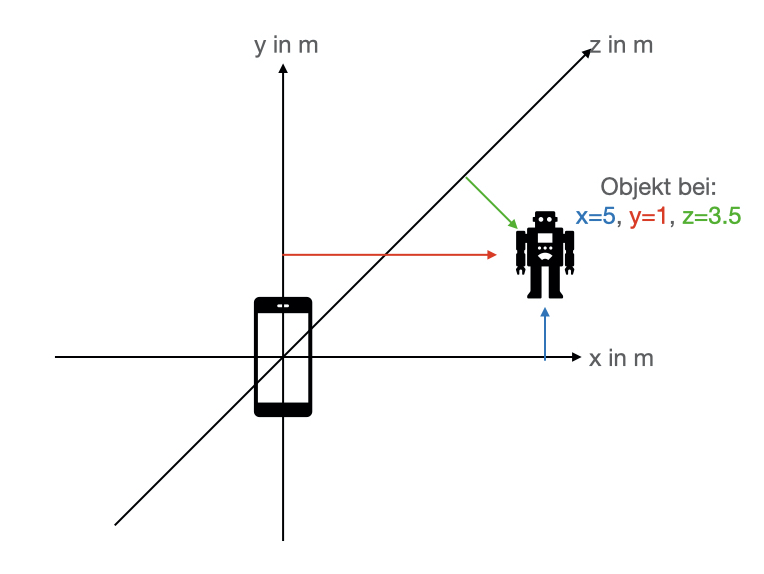
\includegraphics[width=10cm,height=10cm,keepaspectratio]{4Umsetzung/Bilder/koordin.jpeg}
    \caption{Aufbau der Positionsberechnung von Objekten}
    \label{pic:koordin}
\end{figure}
\pagebreak
\\ 
%\linebreak
Beim Setzen eines Objekts wird als Anhaltspunkt der Mittelpunkt des Bildschirms berechnet, um das Objekt auf dem Bildschirm zentriert platzieren zu können. Steht diese 
Position fest, folgt durch Hilfe des \acs{SLAM} Verfahrens die genaue Ermittlung der virtuellen Position. Anhand der Information dieser Position 
ist das Objekt zu platzieren. 
\\ 
Um das Objekte zu setzen, muss der Nutzer in der \acs{UI} (\ref{pic:scan}) im Bereich der „Gallery“ das Objekt anklicken. 
Über die der Sceneform-\acs{API} zur Verfügung gestellten Methode („ModelRenderable“) wird das Objekt erschaffen und als „Anchor“ auf die berechnete Position 
gesetzt. Ein Anchor ist die fixe Position des Objekts, an dem dies platziert wird und so lange dort vorhanden bleibt, bis die Applikation beendet wird. Die Datei, 
die als dreidimensionales „asset“ generiert werden soll, wird über die „uri“-Variable lokalisiert und als Parameter übergeben. 
\\
\begin{lstlisting}[language=C,
    frame=lines,           % Ein Rahmen um den Code (single for box, lines for top and bottom)
    xleftmargin=\parindent,  % Rahmen link von den Zahlen
    style=algoBericht,
    label={code:modelrenderable},
    captionpos=b,           % Caption unter den Code setzen
caption={ModelRenderable Builder}]
ModelRenderable.builder()
.setSource(owner.get(), uri)
.build()
.handle((renderable, throwable) -> {
    ...
}
\end{lstlisting}                                    % (\ref{pic:createObject})
Während der Objekt-Renderung öffnet sich die \acs{GUI} zur Eingabe der Informationen, die sich auf das Objekt beziehen. Diese 
werden dann zusammen mit der virtuellen Position des Objekts abgegriffen und in die Datenbank geschrieben. Speichert der Anwender die Daten über einen Befehl ab, 
%Drückt der Anwender den „save“-Button der Oberfläche 
%(\ref{pic:createObject}), 
beendet er diesen Vorgang und kehrt auf die \acs{UI} der Scan-Phase zurück, um weitere Objekte platzieren zu können. 
\\ 
Zusätzlich zu der Position des Objekts wird dessen Rotation durch Quaternionen berechnet und in der Datenbank gespeichert, um anhand der Berechnung 
die Darstellung so real wie möglich wiederzugeben. Da die Rotation ausgehend von der Kamerahaltung berechnet wird, wird das Objekt bei der Ankerung immer in 
Blickrichtung der Kamera positioniert.
%--> Problemschilderung der Speicherung der Session 
\\ 
\linebreak
Ursprünglich war geplant, die generierte Session sowie die darin erstellten Objekte in der Datenbank abzuspeichern, um diese bei erneutem Aufruf der 
Scan-Phase, bzw. bei Anwendung der Visualisierungs-Phase zu laden und innerhalb dieser Session wieder anzeigen zu lassen. Da die Datenbank nur gewisse Datentypen 
zulässt, war die erste auftretende Schwierigkeit, die Speicherung der Session als Objekt, die zunächst in eine „BLOB“-Datei hätte konvertiert werden müssen. Eine 
„BLOB“-Datei ist ein Binary Large Object, welche anhand der Binärcodierung abgespeichert wird. Dabei kann es sich unter anderem um große 
Bild- oder Audio-Dateien handeln, ebenso können auch mittels dieser Objekt-Konvertierung anderweitig große Dateien gespeichert werden. Daraus entstand in der Visualisierungs-Phase die 
Konsequenz, dass eine erzeugte Session nur eine gewissen Zeit verwendet werden kann. Dies bedeutet, dass nach erneutem 
Starten des Assistenzsystems alle zuvor erzeugten Objekte einer Session auf der ihnen zugewiesenen Position nicht mehr gültig sind. Durch die unterschiedlichen 
Startpunkte, die bei wiederholtem Starten der Anwendung erzeugt werden würden, würde sich die ursprüngliche Ausgangsposition der Applikation verschieben und so auch 
die Objekte an eine fälschliche Position projizieren. Genauer gesagt, müssten die Objekte dann ausgehend von dem neu erzeugten Startpunkt referenziert werden. Somit wäre das 
Ergebnis nicht exakt und könnte keine Anwendung finden, da die Applikation Informationen anzeigen würde, die der Realität nicht entsprechen würden. 
\\ 
Basierend auf dieser Erkenntnis musste umdisponiert und ein neuer Lösungsansatz konzipiert werden. Mit dem Wissen über den aktuellen Stand der ARCore \acs{API} 
galt es eine Lösung zu entwickeln, mit der Positionsinformationen exakt wiedergegeben werden können. 
%\\ 
%Dieser Ansatz wird nun erläutert.
\\ 
\linebreak
Die Idee war es, einen Fixpunkt zu erstellen, welcher dazu dienen würde, einen immer gleichbleibenden Startpunkt vorzugeben. Dadurch gäbe es keine Unterschiede des 
Ausgangspunktes mehr und der Nutzer könnte trotz seiner aktuellen Position die Anwendung starten. Dazu müsste er beim Start der Applikation an den Ursprungspunkt kehren, 
um daraufhin die Scanfunktion zu beginnen. Für diesen Ansatz würde ein Marker zur Verfügung gestellt werden (siehe Abbildung \ref{pic:initialMarker}), der vor dem ersten 
Gebrauch der Software vom Nutzer an einer Position angebracht wird und an dieser dauerhaft bestehen bleibt. Somit ist ein immer gleichbleibender Ausgangspunkt geschaffen, 
von dem aus die Objekte referenziert werden können. Der durch die Anwendung bestimmte Marker müsste entweder als tatsächliches Bild an einer bestimmten Stelle in der 
Realität angebracht werden oder als Bild-Datei auf einem Computer immer vorhanden und an der richtigen Position wiederzufinden sein, um die Genauigkeit zu 
gewährleisten. 
\begin{figure}[hbt!]
    \centering
    
\includegraphics[width=5cm,height=5cm,keepaspectratio]{4Umsetzung/Bilder/cjt_logo_tracking.png}
    \caption{Marker zur Erkennung der Ausgangsposition}
    \label{pic:initialMarker}
\end{figure}
\\
Zur Umsetzung war es notwendig, damit ein Marker verfolgt werden kann, eine weitere Funktion zur Applikation hinzuzufügen (siehe Abbildung \ref{pic:image_tracking} 
in Scan-Phase \ref{chap:scan_implementation} Frontend). Wird dieser Marker erkannt, folgt die eigentliche Scan-Phase, 
die nach der Umkonzeptionierung sowohl bei der Objektplatzierung als auch bei der Datenspeicherung ebenso überarbeitet wurde. 
\\ 
\linebreak
Angenommen der Nutzer startet die Applikation an einer beliebigen Position im Raum und platziert Objekte an von ihm vorgesehene Stellen, dann würden die 
Objekte erstellt, aber keinerlei Anhaltspunkte geschaffen werden, um bei nachzutragenden Objekten die gleichen Voraussetzungen des zu referenzierenden Standpunktes 
zu erfüllen. Daher wird bei der Scan-Phase die Methode zur Markererkennung eingebaut, um einen initialen Fixpunkt anzulegen. Dadurch wird gewährleistet, 
dass ausgehend von diesem Punkt unabhängig vom Start der Applikation erneut Objekte platziert werden können. Demnach werden die Objekte immer abhängig zur 
Position des Fixpunktes gespeichert, erstellt und angezeigt, was bedeutet, dass ein Objekt immer eine Referenz zu dem initialen Marker ist. Auch wenn 
ein Objekt nachträglich hinzugefügt werden soll, muss lediglich der Marker eingescannt werden. Damit ein Objekt an dem vom Nutzer gewünschten Ort platziert 
werden kann, muss er an die Stelle im realen Raum laufen. %Danach begibt sich der Nutzer an den gewünschten Ort im 
%realen Raum, an dem das Objekt in der Anwendung platziert werden soll. 
Jetzt muss er die Umgebung mit der Kamera aufnehmen und, indem er auf den Button für das 
Erstellen des Objekts drückt, dieses virtuell erschaffen. Bei der Erzeugung wird die Position ermittelt und anhand dieser die Differenz, bzw. der 
Abstand zu dem initialen Marker in der Datenbank über einen Schreibbefehl gespeichert. Die Berechnung der Distanz zwischen Objekt und 
Ursprungsmarker erfolgt durch eine Subtraktion, bei der lediglich die Ursprungskoordinaten von den aktuellen Positionskoordinaten subtrahiert werden. 
Dieser Vorgang ist dem folgenden Code-Beispiel (\ref{code:differencetoinitial}) zu entnehmen. Dabei wird das aktuelle Objekt „object“ und das initiale Objekt 
„initialObject“ als Parameter übergeben, %die sogenannte „call by Reference“, 
um die Distanz berechnen zu können. Das Ergebnis wird in mehreren lokalen Variablen 
zwischengespeichert und zum Schluss in eine neue Position „Pose“ mit Translation und Rotation, von der Berechnung durch Quaternionen, ermittelt. Der Rückgabewerte 
dieser Funktion ist demnach eine „Pose“, die nach Aufruf der Methode übergeben und so in der Datenbank mittels „insert“-Befehl hinterlegt wird. 
Die Position und Rotation des einzelnen Objekts ist mit dem Resultat gegeben und kann in der Visualisierungs-Phase verwendet werden.
\\
%\linebreak
\begin{lstlisting}[language=C,
    frame=lines,           % Ein Rahmen um den Code (single for box, lines for top and bottom)
    xleftmargin=\parindent,  % Rahmen link von den Zahlen
    style=algoBericht,
    label={code:differencetoinitial},
    captionpos=b,           % Caption unter den Code setzen
caption={Berechnung der Distanz zwischen Marker und Ursprungspunkt}]
public Pose returnValueFromPosition(Object object, Object initialObject){
    float tX = object.getTx() - initialObject.getTx();
    float tY = object.getTy() - initialObject.getTy();
    float tZ = object.getTz() - initialObject.getTz();

    float qX = object.getQx() - initialObject.getQx();
    float qY = object.getQy() - initialObject.getQy();
    float qZ = object.getQz() - initialObject.getQz();
    float qW = object.getQw() - initialObject.getQw();

    float[] rotation = {qX,qY,qZ,qW};
    float[] translation = {tX,tY,tZ};

    return new Pose(translation, rotation);
}
\end{lstlisting}
Zur Veranschaulichung der zuvor beschriebenen Methodik dient die Abbildung (\ref{pic:differenztoinitial}). Durch diese Skizze wird nochmals verdeutlicht, dass 
sich alles in einem erstellten Koordinatensystem abspielt und lediglich die Distanz der einzelnen Objekte zum Marker berechnet und in der Datenbank persistiert 
werden.
\begin{figure}[hbt!]
    \centering
    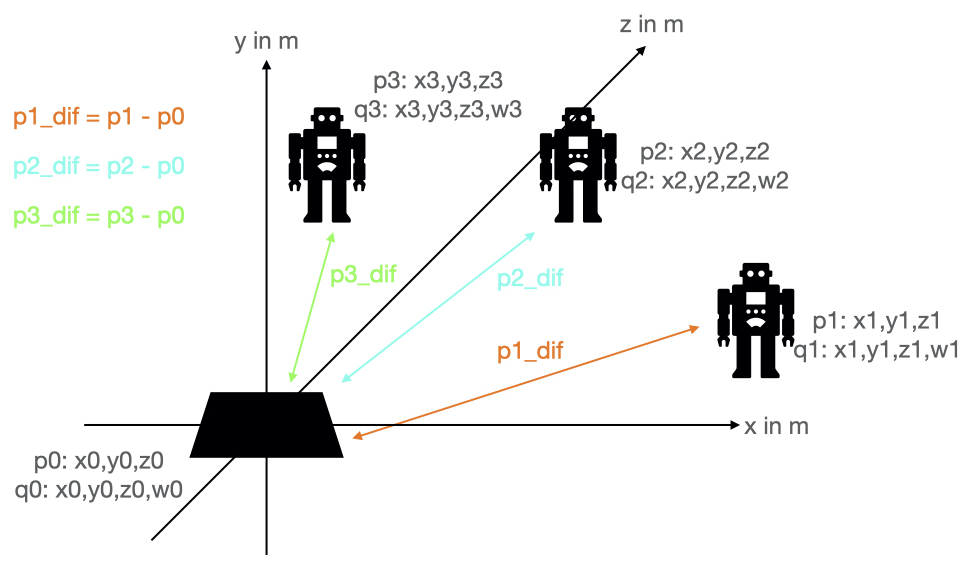
\includegraphics[width=10cm,height=10cm,keepaspectratio]{4Umsetzung/Bilder/difcalc.jpeg}
    \caption{Positionsberechnung zum Ursprungsmarker}
    \label{pic:differenztoinitial}
\end{figure}
%\pagebreak
\\ 
%\linebreak
Um die Backend-Implementierung zu demonstrieren, wird nun während der Laufzeit anhand erstellter Screenshots eine Beschreibung des Ablaufs der Applikation stattfinden.
\\ 
In Abbildung (\ref{pic:markerTracking} (a)) ist zu sehen, dass der vorgegebene Marker verfolgt werden muss, um die Applikation starten zu können. Dabei begrenzt 
die hervorgehobene Umrandung die Fläche, in der der Marker im Bildschirm zur Bildregistrierung platziert werden muss. Nach der Erkennung des Bildes, 
leitet die Benutzeroberfläche automatische auf die eigentliche Ansicht der Scan-Phase um. Ist der Scan aktiviert, folgt die Wahrnehmung der Umgebung durch das 
\acs{SLAM} Verfahren und die Berechnung der vorliegenden Oberflächen. Damit die zu setzenden Objekte exakt auf der Oberfläche des Gegenstandes, der Wand oder dem 
Boden platziert werden können, wird anhand der Sensoren im Smart-Device und dessen Kamera dieser dort berechnet. Dazu wird die berechnete Fläche mit einem Feld voller 
Punkte auf dem Bildschirm überlagert, um dem Nutzer ersichtlich zu machen, 
dass an dieser Position die Schätzung der Oberfläche durchgeführt wurde und die Anwendung darauf ein Objekt platzieren kann. Um dies zu verdeutlichen, wird inmitten 
des Bildschirmes (siehe Abbildung \ref{pic:markerTracking} (b)) ein grüner Punkt angezeigt, der die Platzierung des Objektes vorgibt und dem Nutzer verständlich macht, 
dass ein Objekt erzeugt und an dieser Stelle angesiedelt werden kann. Ist eine Oberfläche der Umgebung noch nicht vollständig berechnet, bzw. erkannt, fehlen 
die Punkte auf dem Bildschirm und es ist lediglich ein grau hinterlegtes Kreuz zu erkennen. Der Nutzer wird dadurch daran gehindert, ein Objekt an einer nicht bekannten 
und nicht berechneten Stelle zu platzieren. 
\begin{figure}[hbt!]
    \centering
    \subfigure[Marker-Scan]{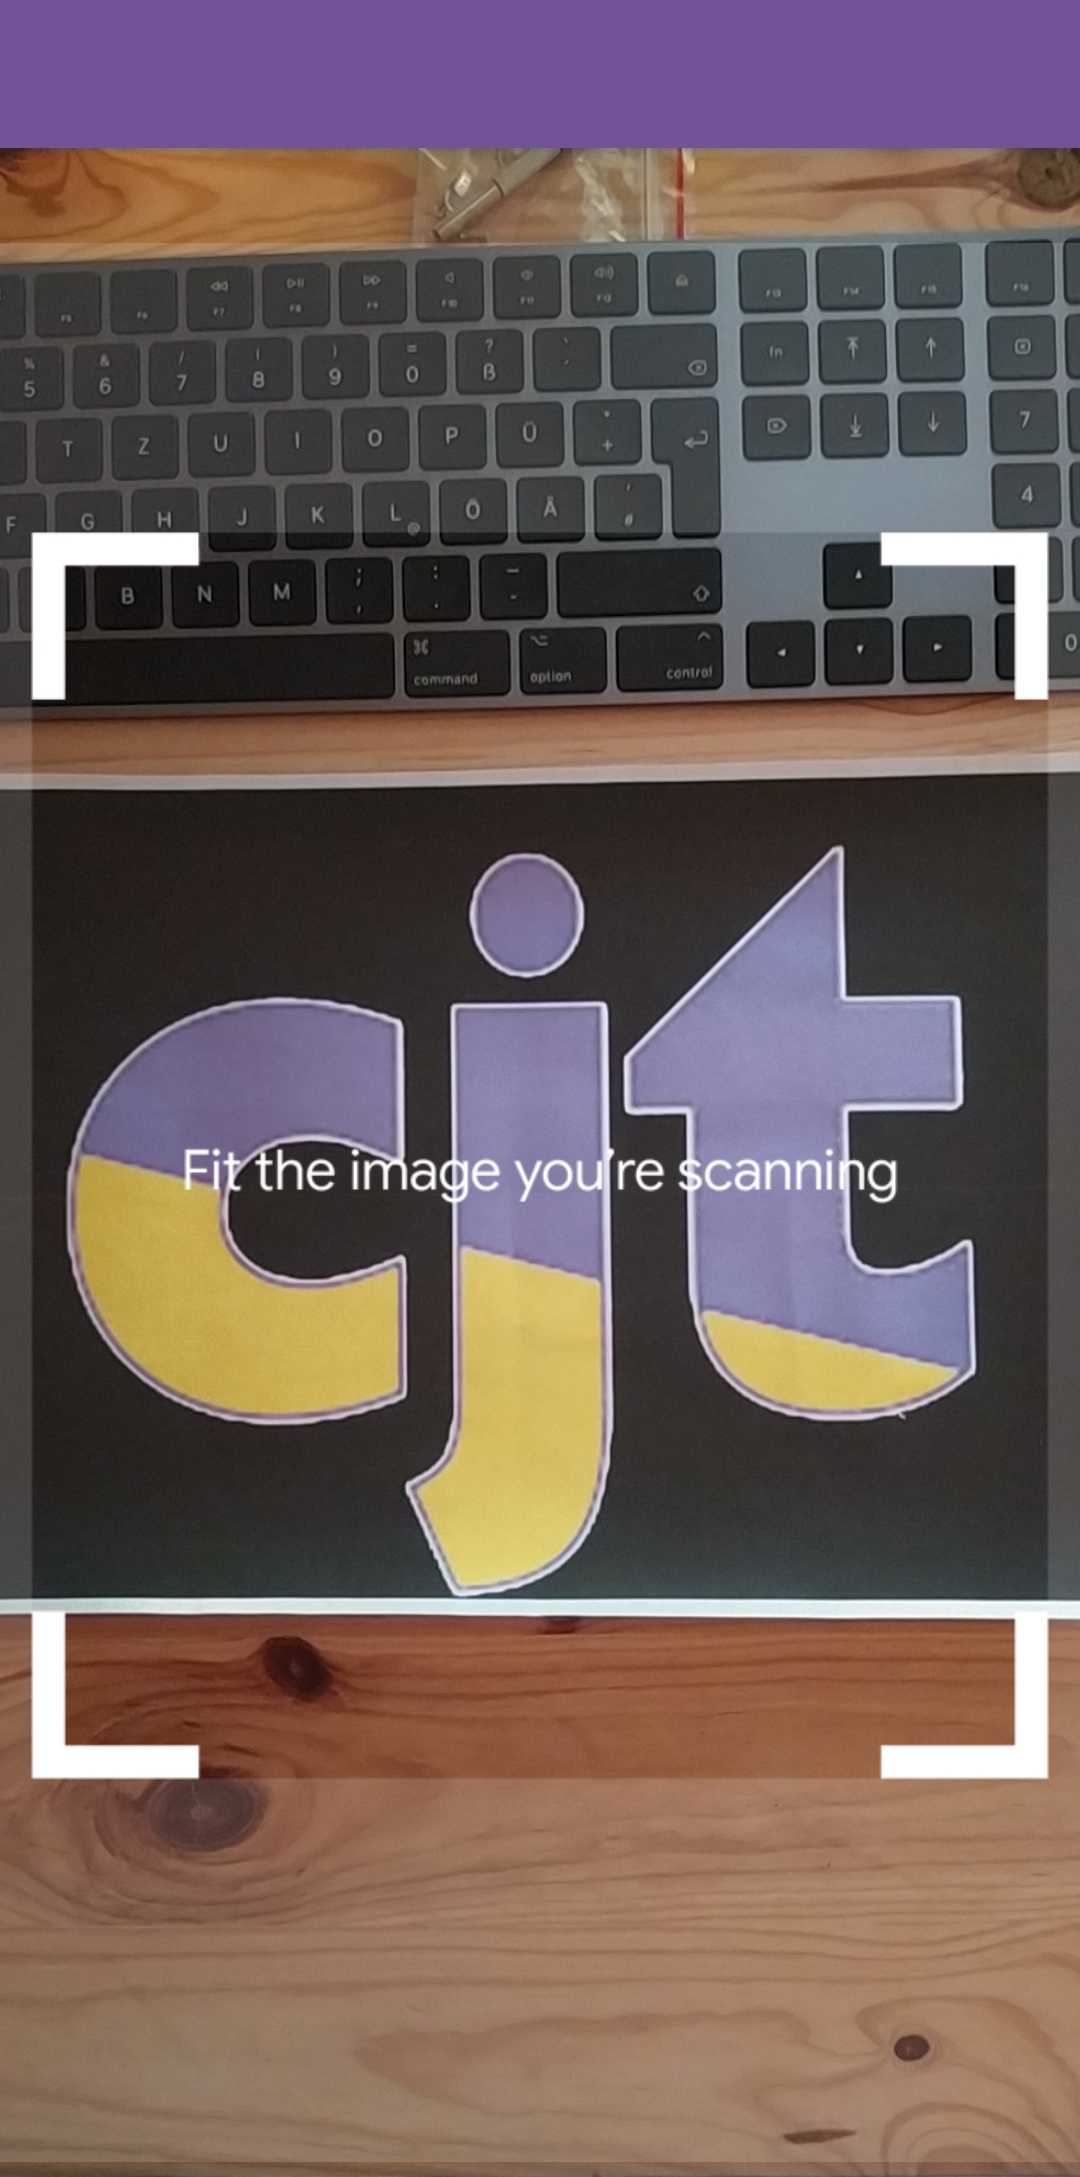
\includegraphics[width=7cm,height=7cm,keepaspectratio]{4Umsetzung//Bilder/scan_image.jpg}}
    \subfigure[Umgebungsberechnung]{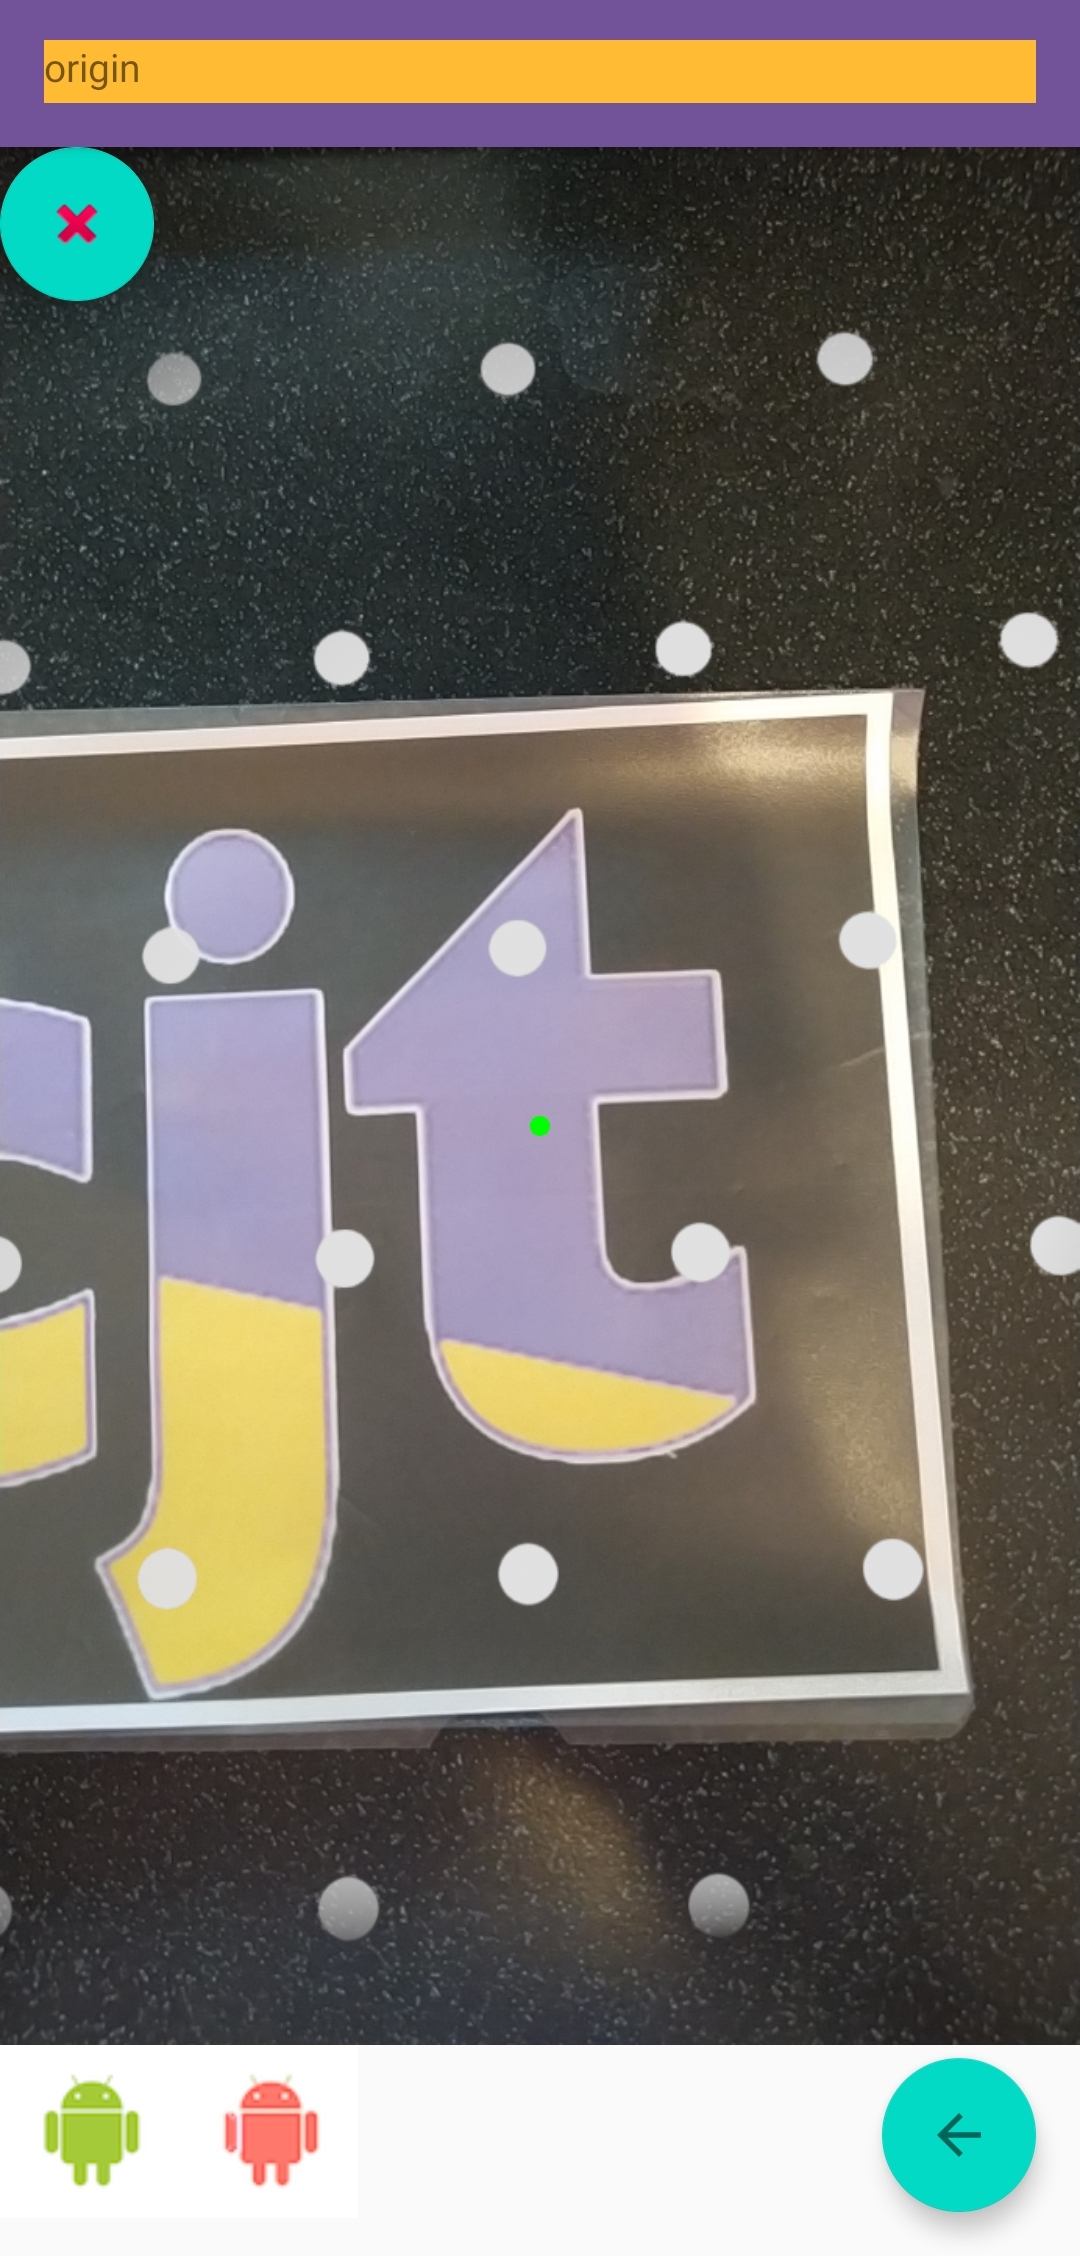
\includegraphics[width=7cm,height=7cm,keepaspectratio]{4Umsetzung/Bilder/scan_environment.jpg}}
    \caption{Funktion der Scan-Phase Teil 1}
    \label{pic:markerTracking}
\end{figure} 
\\ 
Damit ein Objekt vom Benutzer erstellt und an eine von ihm gewählte Position platziert werden kann, muss er die dazugehörigen Informationen in die \acs{UI} 
eintragen und diese bestätigen. Er übernimmt dadurch die Garantie, das Objekt richtig positioniert und betitelt zu haben. Zur weiteren Abfolge des Programms 
wird die ursprüngliche \acs{UI} der Scan-Phase geöffnet und das zuvor erstellte Objekt an der vorgesehenen Stelle platziert. 
Weitere Objekterzeugungen können daraufhin erfolgen, indem ein neuer Ort gewählt und ein Objekt angelegt wird. Die folgende Abbildung demonstriert die 
Darstellung solcher Objekte. Dabei wurden willkürlich 
„Assets" gewählt, die bei tatsächlicher Anwendung in realem Szenario angepasst werden sollten. Die aktuell verwendeten Objekte fungieren lediglich als 
Veranschaulichung der Aktionen und der Repräsentation des Status eines Objekts. Der Abbildung (\ref{pic:place_objects}) ist die Erstellung und 
Darstellung solcher Objekte zu entnehmen. 
\\ 
\linebreak
Über den Button rechts unten verlässt der Nutzer die Scan-Phase nach Platzierung aller Objekte und kann zwischen dem Starten aller Funktionen oder der Beendigung 
der Anwendung wählen. Hat der Nutzer alle gewünschten Objekte platziert, kann dieser über den Button, rechts unten, die Funktion der Scan-Phase verlassen und die 
Visualisierungs-Phase starten oder die Anwendung schließen. Da alle eingegebenen Informationen persistiert sind, gehen diese nicht verloren und können jederzeit 
über die Visualisierungs-Phase aufgerufen werden. Ist dem Nutzer allerdings ein Fehler bei der Erstellung der Objekte unterlaufen, hat er nach aktuellem Stand 
die Möglichkeit, alle vorhandenen Objekte und Daten zu löschen und die Scan-Phase von Anfang an erneut zu starten.  
\begin{figure}[hbt!]
    \centering
    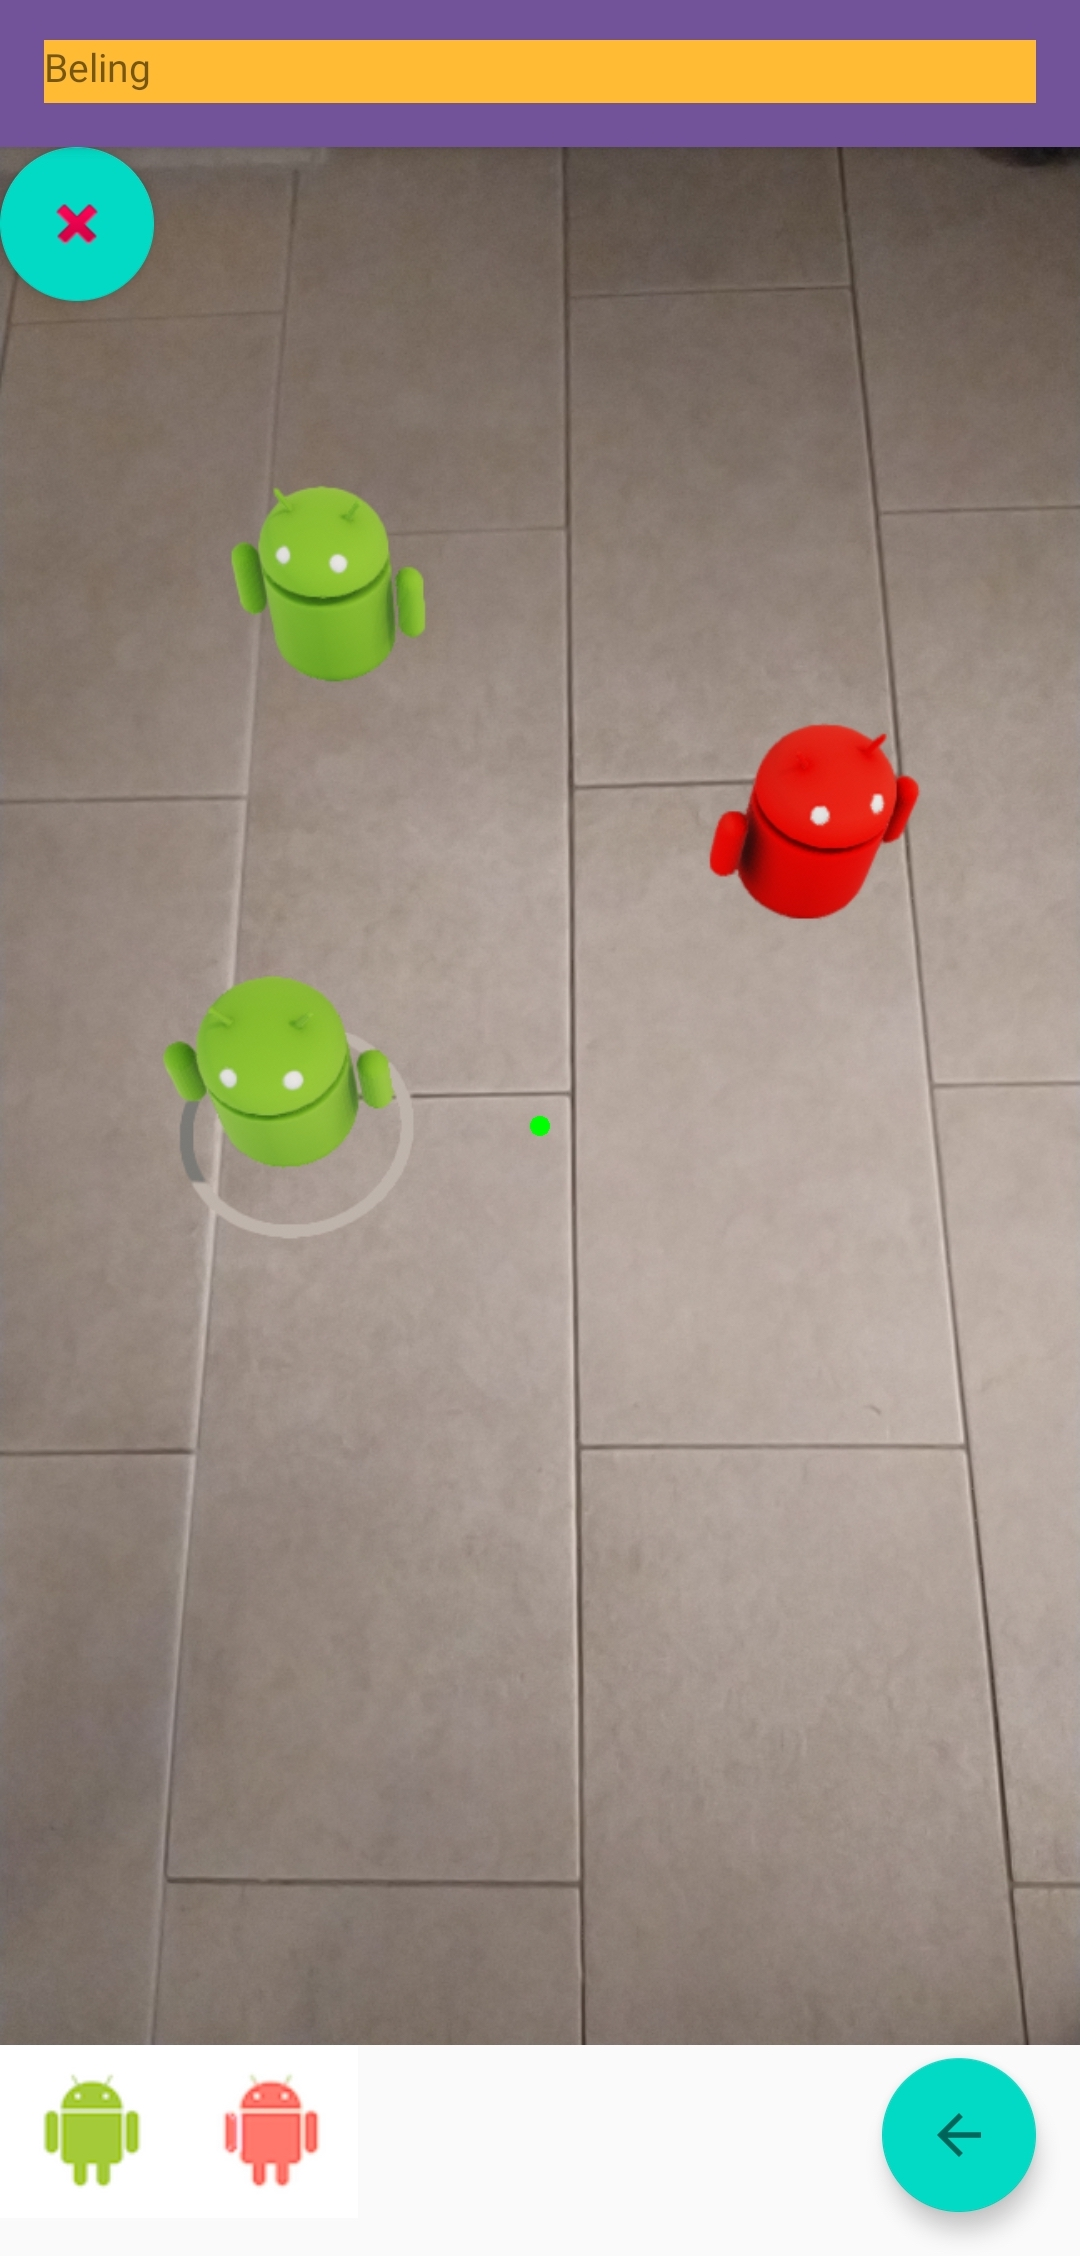
\includegraphics[width=7cm,height=7cm,keepaspectratio]{4Umsetzung/Bilder/place_objects_view.jpg}
    \caption{Funktion der Scan-Phase Teil 2}
    \label{pic:place_objects}
\end{figure}
%\pagebreak
%\\ 
%\linebreak
%Nachdem die Scan-Phase nun vollends beschrieben wurde, geht es in folgendem Kapitel um die Erläuterung des dritten und letzten Use Cases. Dabei werden sowohl 
%ie Frontend als auch die Backend Aspekte aufgezeigt. Ebenso wird die Funktionsweise der Objekt-Repräsentation anhand eines kleinen Beispiels, ähnlich wie bereits in 
%er Scan-Phase erläutert, veranschaulicht.
\subsection{Visualisierungs-Phase} 
Nach vollständiger Beendigung der Scan-Phase ging es in der Entwicklung weiter mit der Visualisierungs-Phase. Die zuvor gespeicherten Objekte und 
deren Informationen werden dabei abgerufen und können jederzeit erneut visualisiert und im Raum platziert werden. Die folgende Darlegung der 
Frontend-Entwicklung der Visualisierungs-Phase gibt Aufschluss über die Benutzeroberfläche dieser Phase und deren Aufbau. %Die Ausführung des Frontends und deren bildliche 
%Darstellung dient dazu, das anschließende Backend nachvollziehen zu können. Abschließend werden die Aspekte des Frontends aufgegriffen und anhand der Backend-Implementierung 
%mit deren Funktionen verknüpft. 

\subsubsection{FrontEnd}
Bei der Visualisierungs-Phase gibt es prinzipiell eine Benutzeroberfläche, die diesen Use Case ausmacht. Unter eigentlicher Anwendung dieser Phase und 
deren \acs{GUI} befinden sich darüber hinaus weitere Benutzeroberflächen, die bereits in der Scan-Phase schon erläutert wurden. Darunter zum Beispiel 
die in Abbildung (\ref{pic:image_tracking}) zu entnehmende Markererkennungs-\acs{UI}, die ebenso Bestandteil der Visualisierungs-Phase ist. 
\\ 
Die primäre \acs{GUI} ist ähnlich zu der Benutzeroberfläche der Scan-Phase aufgebaut. 
Ein Fragment, das sich über den ganzen Bildschirm erstreckt, repräsentiert das Livebild der Kamera. Dadurch können die bereits in der Scan-Phase erstellten 
Objekte erneut angezeigt werden und es ist eine überschaubare und leicht zu verstehende Oberfläche gegeben. Des Weiteren befinden 
sich auf dieser Oberfläche zwei Buttons, zum einen zur Navigation, um auf das Startmenü zu gelangen, und zum anderen, um die Objekte von der Datenbank 
abzugreifen, rendern und auf dem Bildschirm anzeigen zu lassen. Diese befinden sich jeweils in der linken und rechten unteren Ecke des Bildschirms, wie 
der Abbildung \ref{pic:visual} zu entnehmen ist. 
Da diese \acs{UI} nur als Ansicht der zu visualisierenden Objekte gedacht ist, stehen dem Nutzer für die Interaktionen nur die Objekte, die als Overlay 
über das Kamerabild gelegt werden, zur Verfügung. Die Nutzeraktionen beschränken sich lediglich auf den Gebrauch der zuvor genannten Buttons und die dynamisch erzeugten 
Schaltflächen der Objekte, um über diese zusätzliche Informationen zu erhalten. 
\begin{figure}[hbt!]
    \centering
    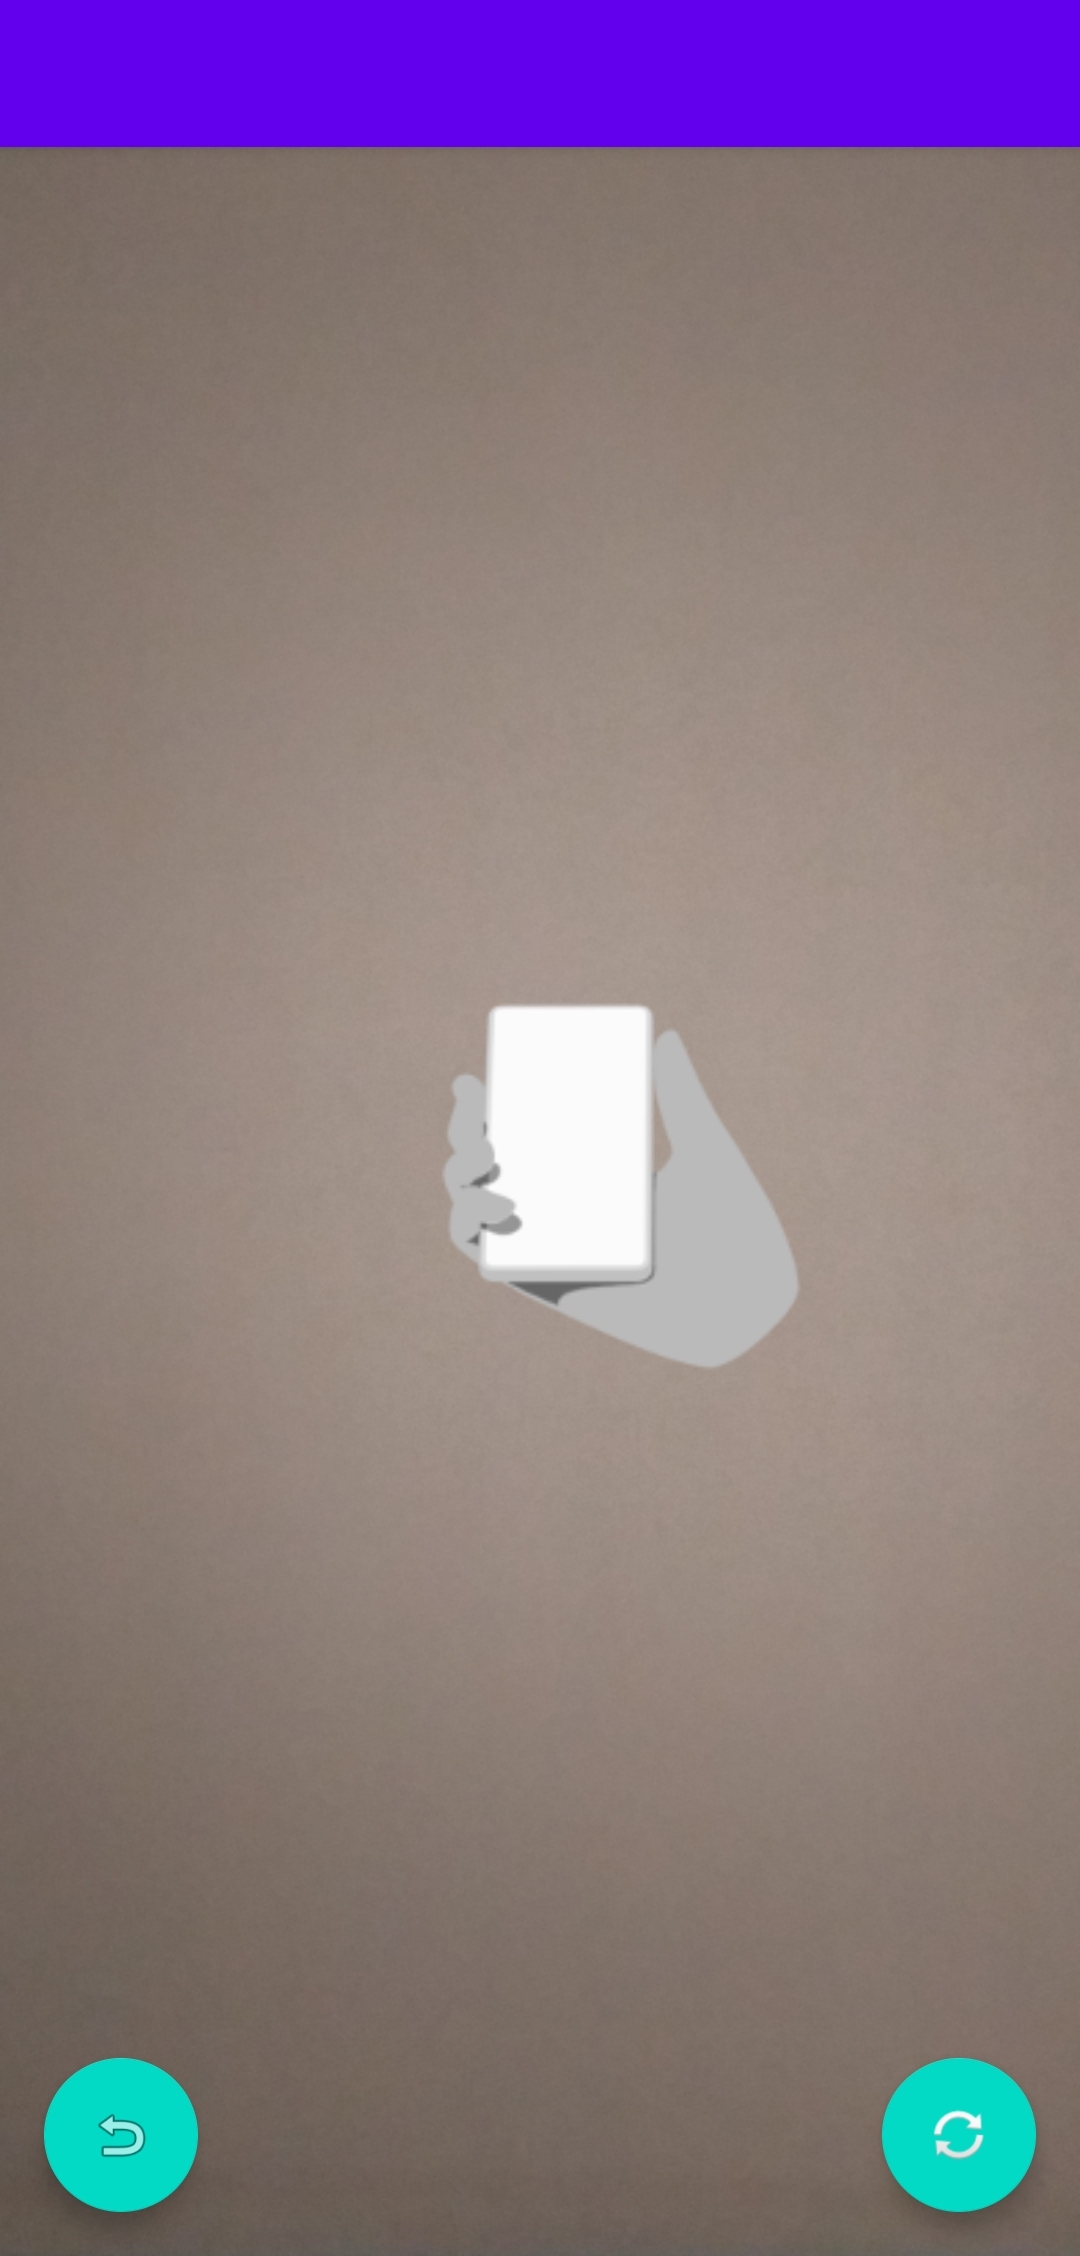
\includegraphics[width=7cm,height=7cm,keepaspectratio]{4Umsetzung/Bilder/visual-phase.jpg}
    \caption{Visualisierungs-Phase der Applikation}
    \label{pic:visual}
\end{figure} 
\\ 
Mit der soeben erläuterten Benutzeroberfläche geht folgender Programmablauf einher. Mit der gewonnenen Kenntnis des Ablaufs kann sich die 
Implementierung des Backends daran stützen. 
\begin{figure}[hbt!]
    \centering
    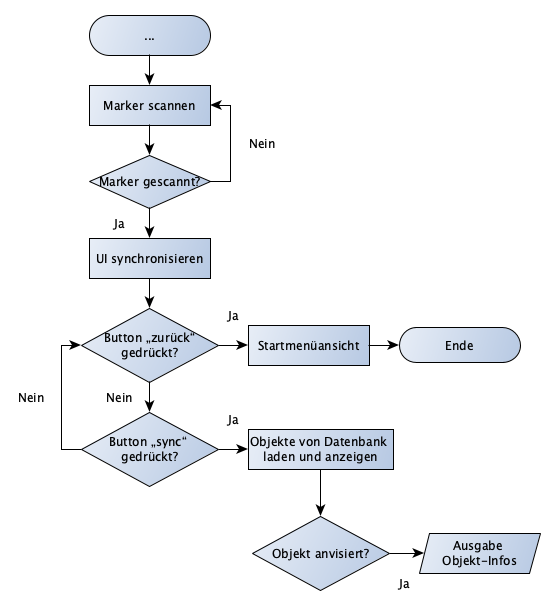
\includegraphics[width=15cm,height=15cm,keepaspectratio]{4Umsetzung/Bilder/visualPAP.png}
    \caption{Programmablaufplan der Visualisierungs-Phase}
    \label{pic:startmenu}
\end{figure}
\pagebreak
\\
%\linebreak
Auf Grundlage der Benutzeroberflächen erfolgt die Beschreibung der Backend-Implementierung und Einblicke in die Programmierung der Visualisierungs-Phase.